\section{Results}
\label{sec:results}
Figure \ref{fig:grafGra} shows the knowledge graph generated by the query shown in listing \ref{lst:script5}. It is appreciated that the rectangles in purple contain the name of the object and those in fuchsia represent the identifier of the object. Each object can have zero or more relationships to other objects\footnote{Strictly, they only relate to objects that are part of the query.}. However, an object unrelated to others is of no use because it could not be reached since it has no edges, which represent ontological relationships. In addition, implicit or explicit information can be extracted through the edges (green lines).

\lstinputlisting[language=Python, firstline=9, lastline=17,
caption=Query to generate the knowledge graph., label={lst:script5}]{code/queries.gql}

\begin{figure}[H]
    \centering
    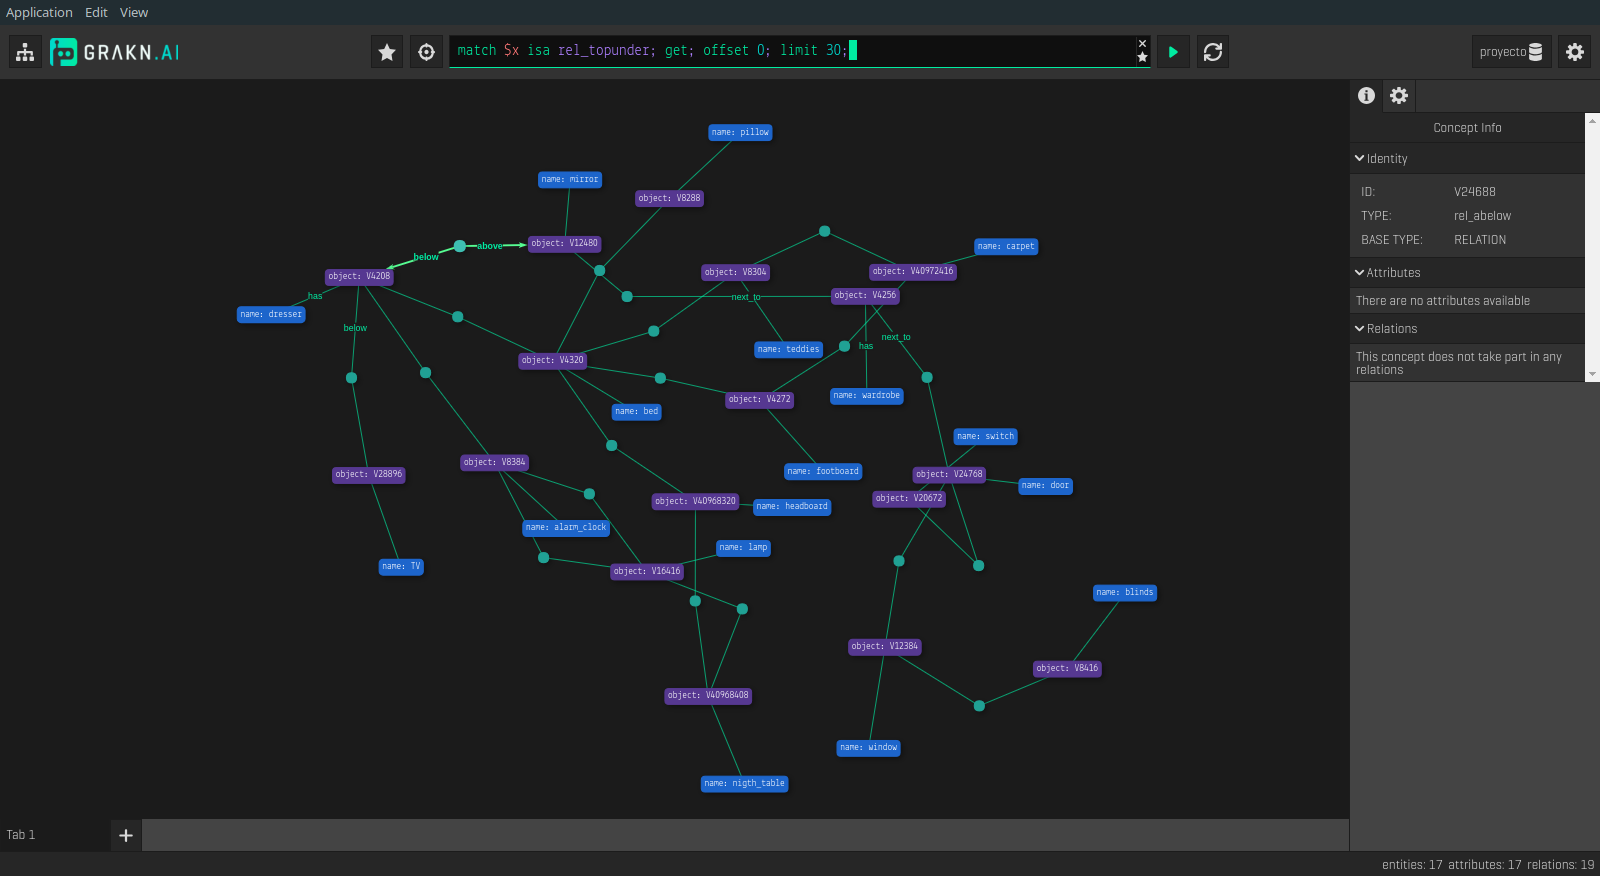
\includegraphics[width=8.8cm]{figures/allrel.png}
    \caption{Knowledge graph in Grakn.}
    % \caption{Grafo en Grakn}
    \label{fig:grafGra}
\end{figure}

The explicit information obtained from the edges explains why the objects were determined to be related. In most cases it is by the nature of the \textit{query} that it is executed. On the other hand, the implicit information is related to the \textit{background} of the relation of objects and is usually used when making inferences, better known as \textit{automatic reasoning}. It is worth mentioning that in this work we only work with explicit relationships.

Figure \ref{fig:ReGra} shows the relationship \textit{rel-topunder} between the bed and footboard which can be expected while finding the object ``footboard'' under the object ``bed'' and the object ``bed'' in top of the ``footboard''. Also, in the same image, the \textit{rel-abelow} relationship between the footboard and carpet can be seen similarly to the previous one.

\begin{figure}[H]
    \centering
    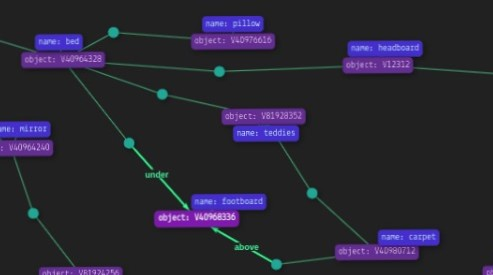
\includegraphics[width=8.4cm]{figures/realcionGrafo.jpeg}
    \caption{Relation bed-footboard, footboard-carpet.}
    % \caption{Relación bed-footboard, footboard-carpet}
    \label{fig:ReGra}
\end{figure}

This work is a contribution to the categorization of the semantic context in computer vision since it establishes the tools and a baseline in spatial relationships to create maps of the environment of places of human occupation, using knowledge graphs, in contrast to the common way it is done.

Normally, to avoid processing an immense quantity of convolutions, which translates into higher execution time, \cite{Galleguillos} suggests creating object context base on object scale or spatial context, by creating big comparison lists (dataset) and contrasting them with image training sets. This is a good approach, however, the list remains static and does not get feedback from the training dataset. Which our model does naturally because that is how knowledge graphs work.